
\subsection*{4.3 Angles of Elevation and Depression, bearing}
Angles of elevation and depression are used to describe the inclination or declination of a line of sight relative to the horizontal plane.

\textbf{Key Concepts:}

\begin{itemize}
	\item \textbf{Angle of Elevation:} The angle between the horizontal line and the line of sight when an observer looks up at an object.
	\item \textbf{Angle of Depression:} The angle between the horizontal line and the line of sight when an observer looks down at an object.
	
\end{itemize}

\textbf{Examples:}

\begin{flushleft}
	\textbf{Example 1: A person standing 50 m away from a tower observes the top of the tower at an angle of elevation of $35^\circ$. Find the height of the tower.}
	
	\vspace{0.5cm}
	\textbf{Solution:}
	\vspace{0.5cm}
	
	Step 1: Identify the known values:
	- The horizontal distance to the tower is 50 m.
	- The angle of elevation is $35^\circ$.
	- The height of the tower is the opposite side.
	
	Step 2: Use the tangent function:
	\[
	\tan 35^\circ = \frac{\text{height}}{\text{distance}}.
	\]
	
	\[
	\tan 35^\circ = \frac{h}{50}.
	\]
	
	Step 3: Solve for $h$:
	\[
	h = 50 \times \tan 35^\circ.
	\]
	
	Using $\tan 35^\circ \approx 0.7002$:
	\[
	h = 50 \times 0.7002 = 35.01 \text{ m}.
	\]
	
	Thus, the height of the tower is approximately $35.0$ m.
\end{flushleft}

\begin{flushleft}
	\textbf{Example 2: A pilot at an altitude of 2 km observes an airport at an angle of depression of $20^\circ$. Find the horizontal distance from the airplane to the airport.}
	
	\vspace{0.5cm}
	\textbf{Solution:}
	\vspace{0.5cm}
	
	Step 1: Identify the known values:
	- The altitude (vertical height) is 2 km.
	- The angle of depression is $20^\circ$.
	- The horizontal distance is the adjacent side.
	
	Step 2: Use the tangent function:
	\[
	\tan 20^\circ = \frac{\text{altitude}}{\text{horizontal distance}}.
	\]
	
	\[
	\tan 20^\circ = \frac{2}{d}.
	\]
	
	Step 3: Solve for $d$:
	\[
	d = \frac{2}{\tan 20^\circ}.
	\]
	
	Using $\tan 20^\circ \approx 0.3640$:
	\[
	d = \frac{2}{0.3640} \approx 5.49 \text{ km}.
	\]
	
	Thus, the horizontal distance is approximately $5.49$ km.
\end{flushleft}

\begin{flushleft}
	\textbf{Example 3: A boat is sailing towards a lighthouse. When the boat is 300 m from the lighthouse, the angle of elevation to the top of the lighthouse is $25^\circ$. If the height of the lighthouse is 60 m, find the distance from the top of the lighthouse to the boat.}
	
	\vspace{0.5cm}
	\textbf{Solution:}
	\vspace{0.5cm}
	
	Step 1: Identify the known values:
	- The horizontal distance is 300 m.
	- The height of the lighthouse is 60 m.
	- The required distance is the hypotenuse.
	
	Step 2: Use the sine function:
	\[
	\sin 25^\circ = \frac{60}{d}.
	\]
	
	Step 3: Solve for $d$:
	\[
	d = \frac{60}{\sin 25^\circ}.
	\]
	
	Using $\sin 25^\circ \approx 0.4226$:
	\[
	d = \frac{60}{0.4226} \approx 142.02 \text{ m}.
	\]
	
	Thus, the distance from the top of the lighthouse to the boat is approximately $142.0$ m.
\end{flushleft}


\begin{flushleft}
	\textbf{Example 3:} The bearing of $Q$ from $P$ is $015^\circ$ and the bearing of $P$ from $R$ is $015^\circ$. If $Q$ and $R$ are $24$ km and $32$ km respectively from $P$:
	
	\begin{enumerate}
		\item[(i)] Represent this information in a diagram.
		\item[(ii)] Calculate the distance between $Q$ and $R$, correct to two decimal places.
		\item[(iii)] Find the bearing of $R$ from $Q$, correct to the nearest degree.
	\end{enumerate}
	
	\vspace{0.5cm}
	\begin{center}
		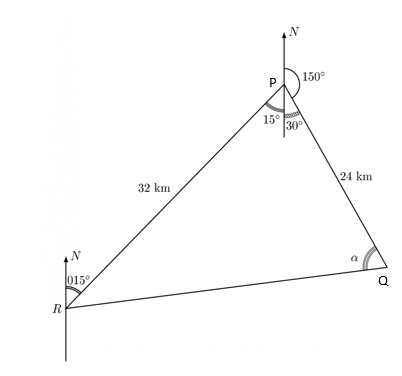
\includegraphics[width=0.6\textwidth]{4.3.png}
	\end{center}
	
	\textbf{Solution:}
	\vspace{0.5cm}
	
	Step 1: Represent the given bearings in a diagram. Since both bearings are measured from the north, we construct a diagram accordingly.
	
	Step 2: Use the cosine rule to find the distance between $Q$ and $R$. The angle between $PQ$ and $PR$ is:
	\[
	\theta = (15^\circ + 35^\circ) = 145^\circ.
	\]
	Using the cosine rule:
	
	\[
	|QR|^2 = 32^2 + 24^2 - 2 \times 32 \times 24 \times \cos 45^\circ
	\]
	
	\[
	|QR|^2 = 1024 + 576 - 1536 \cos 45^\circ
	\]
	
	\[
	= 1600 - 1086.1056
	\]
	
	\[
	|QR|^2 = 513.8944
	\]
	
	\[
	|QR| = \sqrt{513.8944} = 22.669 \text{ km}
	\]
	
	\[
	\approx 22.67 \text{ km to 2 dp} 
	\]
	
	
	
	Step 3: Find the angle \angle PQR using the sine rule:
	\[
	\frac{32}{\sin \angle PQR} = \frac{22.67}{\sin 45^\circ}
	\]
	
	\[
	\sin \angle PQR = \frac{32 \times \sin 45^\circ}{22.67}
	\]
	
	\[
	= 0.9981
	\]
	
	\[
	\angle PQR = \sin^{-1} (0.9981) = 86.4787^\circ
	\]
	
	
	
	Step 4: Calculate the bearing of $R$ from $Q$:
	\\
	\begin{center}
		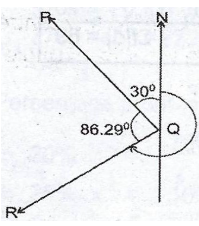
\includegraphics[width=0.6\textwidth]{4.4.png}
	\end{center}
	The bearing of R from Q is given by the reflex angle NQR. Thus,
	
	\[
	\text{Reflex } \angle NQR = 360^\circ - (86.47^\circ + 30^\circ)
	\]
	
	\[
	= 360^\circ - 116.47^\circ
	\]
	
	\[
	= 243.53^\circ
	\]
	
	Hence, the bearing of R from Q:
	
	\[
	\approx 244^\circ \quad (\text{to the nearest degree})
	\]
	
	
\end{flushleft}
